%!TEX root = thesis.tex

\chapter{Data: visual and automated morpholgies}
\label{chap:2}


This chapter presents all data used in this research. It begins with an in depth overview of the Galaxy Zoo 2 project, including the galaxy sample and classification procurement. It then covers in considerable detail the methodology for obtaining the morphological structural indicators measured for the Galaxy Zoo 2 sample. 


%%%%%%%%%%%%%%%%%%%%%%%%%%%%%%%%%%%%%%%%%%%%%%%%%%%%%%%%%%%%%%%%%%%%%%%%%%
%%%		SECTION: 	GALAXY SAMPLE SELECTION
%%%%%%%%%%%%%%%%%%%%%%%%%%%%%%%%%%%%%%%%%%%%%%%%%%%%%%%%%%%%%%%%%%%%%%%%%%
\section{Galaxy Zoo}
Founded by co-creators Chris Lintott and Kevin Schawinksi, Galaxy Zoo is a crowd-sourced innitiative to visually classify large numbers of galaxies by asking members of the general public. It began in 2007 with the classification of 893,212 galaxy images from the Sloan Digital Sky Survey (SDSS) Data Release 6 with $r < 17.77$ Petrosian AB magnitudes \cite{Strauss2002,Adelman2008}. The first iteration of the project was simplistic, inviting volunteers to determine whether a galaxy was elliptical, spiral, or a star / artifact. The project was an immediate success both in terms of the public interest and the resulting science. Following the completion of GZ1 \cite{Lintott2008}, over a dozen peer-reviewed articles utilzing GZ1 classifications\footnote{\url{https://www.zooniverse.org/about/publications}} were published. In addition to explorations of galaxy morphology and its dependence on color and environment \cite{Skibba2009, Bamford2009}, significant results also included substantial populations of red disks \cite{Masters2010b}, blue ellipticals \cite{Schawinski2009}, and discoveries of rare objects such as the ``green peas'' \cite{Cardamone2009}, and Hanny's Voorwerp \cite{Lintott2009}, the first obvservation of a AGN ionization echo. 

The early sucess of GZ1 led to several subsequent and progressively more complex projects. To date, Galaxy Zoo has provided morphologies for over a million galaxies from multiple imaging surveys of various wavebands and redshifts using classifications provided from over a million volunteers. A summary of Galaxy Zoo projects is given in Table XXX. The current research uses data specifically from the Galaxy Zoo 2 (GZ2) project \cite{Willett2013}, the immediate successor of GZ1. The following sections provide an overview of the project specifics including the galaxy sample, the decision tree structure, and a brief description of how volunteer ``clicks'' are converted into useful classifications. 


%%%%%%%%%%%%%%%%%%%%%%%%%%%%%%%%%%%%%%%%%%%%%%%%%%%%%%%%%%%%%%%%%%%%%%%%%%
%%%		SUBSECTION:		GALAXY SAMPLE SELECTION
%%%%%%%%%%%%%%%%%%%%%%%%%%%%%%%%%%%%%%%%%%%%%%%%%%%%%%%%%%%%%%%%%%%%%%%%%%
\subsection{Galaxy sample selection}
The original GZ1 project sought broad classifications for nearly one million galaxies in SDSS. Due to the sheer number of galaxies to quantify, the morphologies collected were broad, seeking to determine between early-type, late-type and mergers. However, much can be gained by probing more detailed morpholgies such as the existance of bars, bulges, dust lanes, rings, etc. Galaxy Zoo 2 thus selected the nearest and brightest 25\% of galaxies from the original GZ1 sample, galaxies for which fine morphological structure could be resolved and classified. Pulled from Data Release 7 Legacy catalog \cite{Abazajian2009} which imaged the the North Galactic Cap, this galaxy sample required the Petrosian half-light magnitude be brighter than 17.0 in the r-band, along with a size limit such that petror90\_r $>3$, where petror90\_r is the radius containing 90\% of the r-band Petrosian aperture flux. Spectroscopic redshifts were pulled from the SDSS Main Galaxy Sample \cite{Strauss2002} and galaxies outside of $0.0005 < z < 0.25$ were removed, though objects without reported redshifts remained in the sample. This resulted in a sample of 273,783 galaxies. 

In addition to the DR7 Legacy catalog, galaxies were included from Stripe 82, a multipy-imaged strip along the celestial equator in the Southern Galactic Cap. Galaxies in this region were selected to have $m_r\le17.7$. GZ2 included multiple sets from this region: a set of 21,522 single-exposure images (though only about half conformed to the shallower Legacy magnitude cut specified above), and two sets of $\sim$30K co-added images from multiple exposures resulting in an object detection limit approximately two magnitudes deeper than the normal depth imaging. The research presented in this thesis utilizes the final GZ2 single-depth sample consisting of 295,305 galaxies of which 11,334 have the deeper magnitude limit. 


%%%%%%%%%%%%%%%%%%%%%%%%%%%%%%%%%%%%%%%%%%%%%%%%%%%%%%%%%%%%%%%%%%%%%%%%%%
%%%		SUBSECTION:		GZ2 DECISION TREE / PROJECT HISTORY
%%%%%%%%%%%%%%%%%%%%%%%%%%%%%%%%%%%%%%%%%%%%%%%%%%%%%%%%%%%%%%%%%%%%%%%%%%
\subsection{GZ2 decision tree and project history}
Using GZ2 nomenclature, a \textit{classification} is the total amount of information about a subject obtained by completing all tasks in the decision tree. Each step in the tree is a \textit{task} consisting of a \textit{question} and a set of \textit{responses}. A volunteer's response is referred to as a \textit{vote}. With the exception of the first question, subsequent tasks depended on the response to the current question. The first question in the tree is a modification of the GZ1 project, asking volunteers to identify whether a galaxy is `smooth', has `features or a disk', or is a `star or artifact'. The full decision tree is shown in Figure \ref{fig: gz2 decision tree}. Volunteers are allowed to select a single option for each question and are immediately taken to the next task after responding. 

%%%%%%%%%%%%%%%%%%%%%%%%%%%%%%%%%%%%%%%%%%%%%%%%%%%%%%%%%%%%%%%%%%%%%%%%%%
%%%		FIGURE: 	GZ2 DECISION TREE
%%%%%%%%%%%%%%%%%%%%%%%%%%%%%%%%%%%%%%%%%%%%%%%%%%%%%%%%%%%%%%%%%%%%%%%%%%
\begin{figure}[h!]
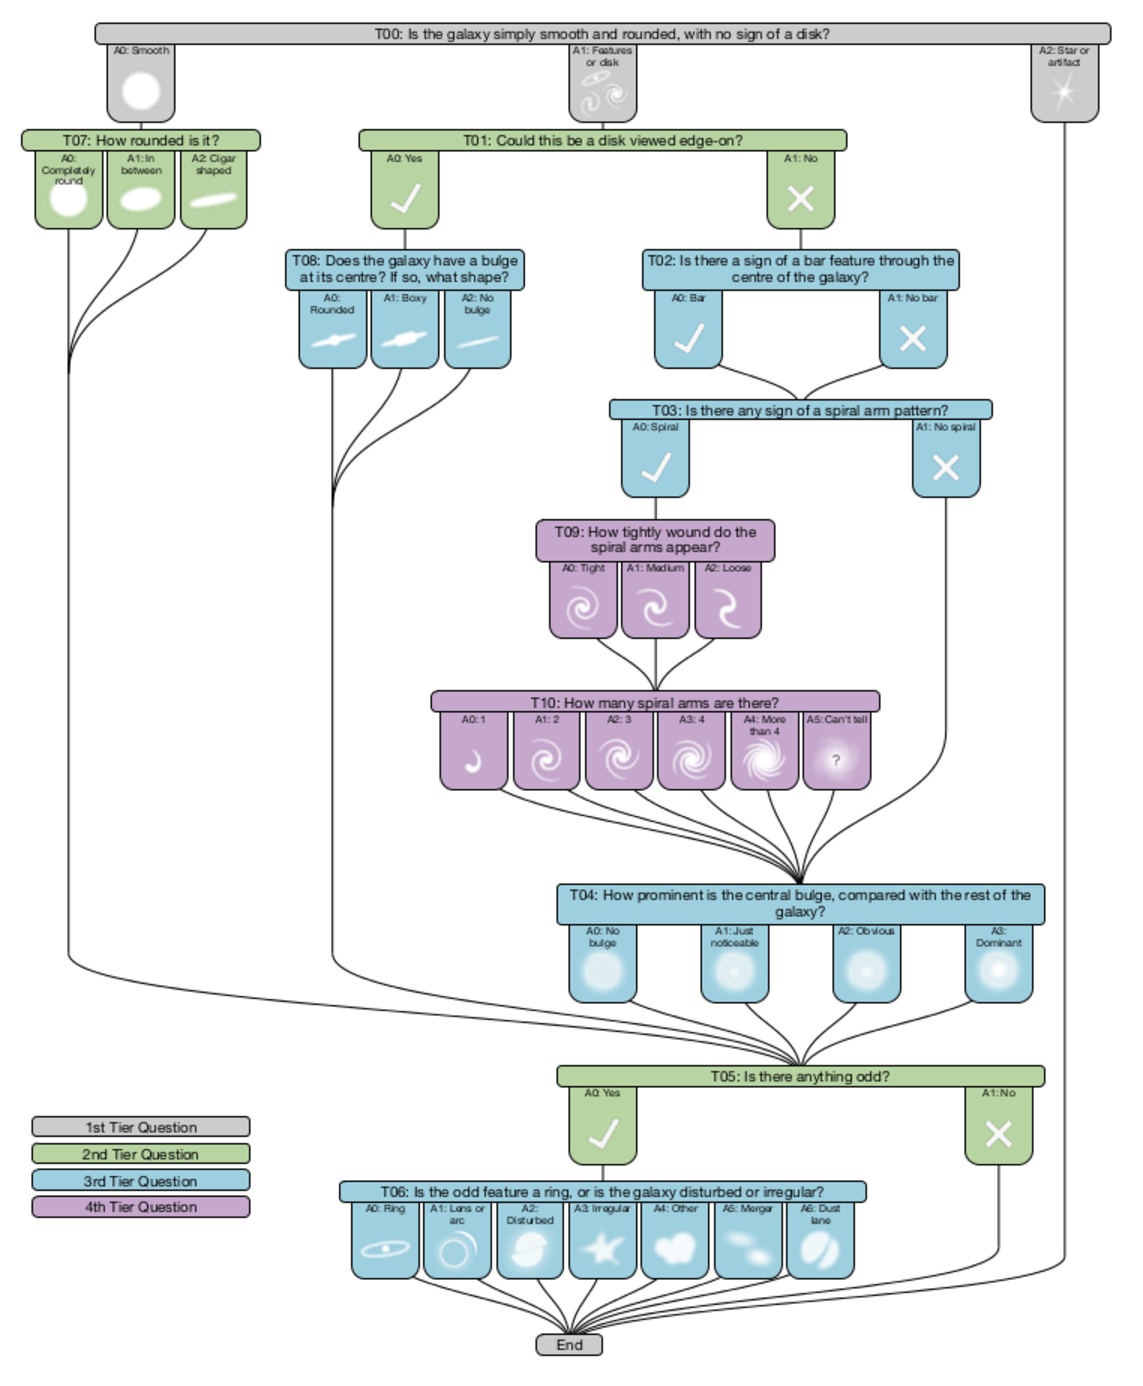
\includegraphics[width=\textwidth]{Figures/gz2_tree.pdf}
\caption{AHMAH MUTHAFUCKIN CAPTION BITCHES}
\label{fig: gz2 decision tree}
\end{figure}

For the single-depth sample, volunteers were shown color images generated from the SDSS ImgCutout web service. Each image is a $gri$ color composite scaled to $0.02\times$petror90\_r. Throughout the life of GZ2 these images were drawn randomly with the exception that towards the end of the project, galaxy images with few responses were shown more frequently in order to ensure that each galaxy had a sufficient number of classifications to adequately charactrize the likelihood of the classification distribution. This resulted in a median of 44 classifications per galaxy with a wide spread (Show Kyle's figure?). The full project spanned just over 14 months with the final dataset consisting of over 16 million classifications from over 80 thousand volunteers. 
 
%%%%%%%%%%%%%%%%%%%%%%%%%%%%%%%%%%%%%%%%%%%%%%%%%%%%%%%%%%%%%%%%%%%%%%%%%%
%%%		FIGURE: 	GZ2 WEB INTERFACE
%%%%%%%%%%%%%%%%%%%%%%%%%%%%%%%%%%%%%%%%%%%%%%%%%%%%%%%%%%%%%%%%%%%%%%%%%%
\begin{figure}[h!]
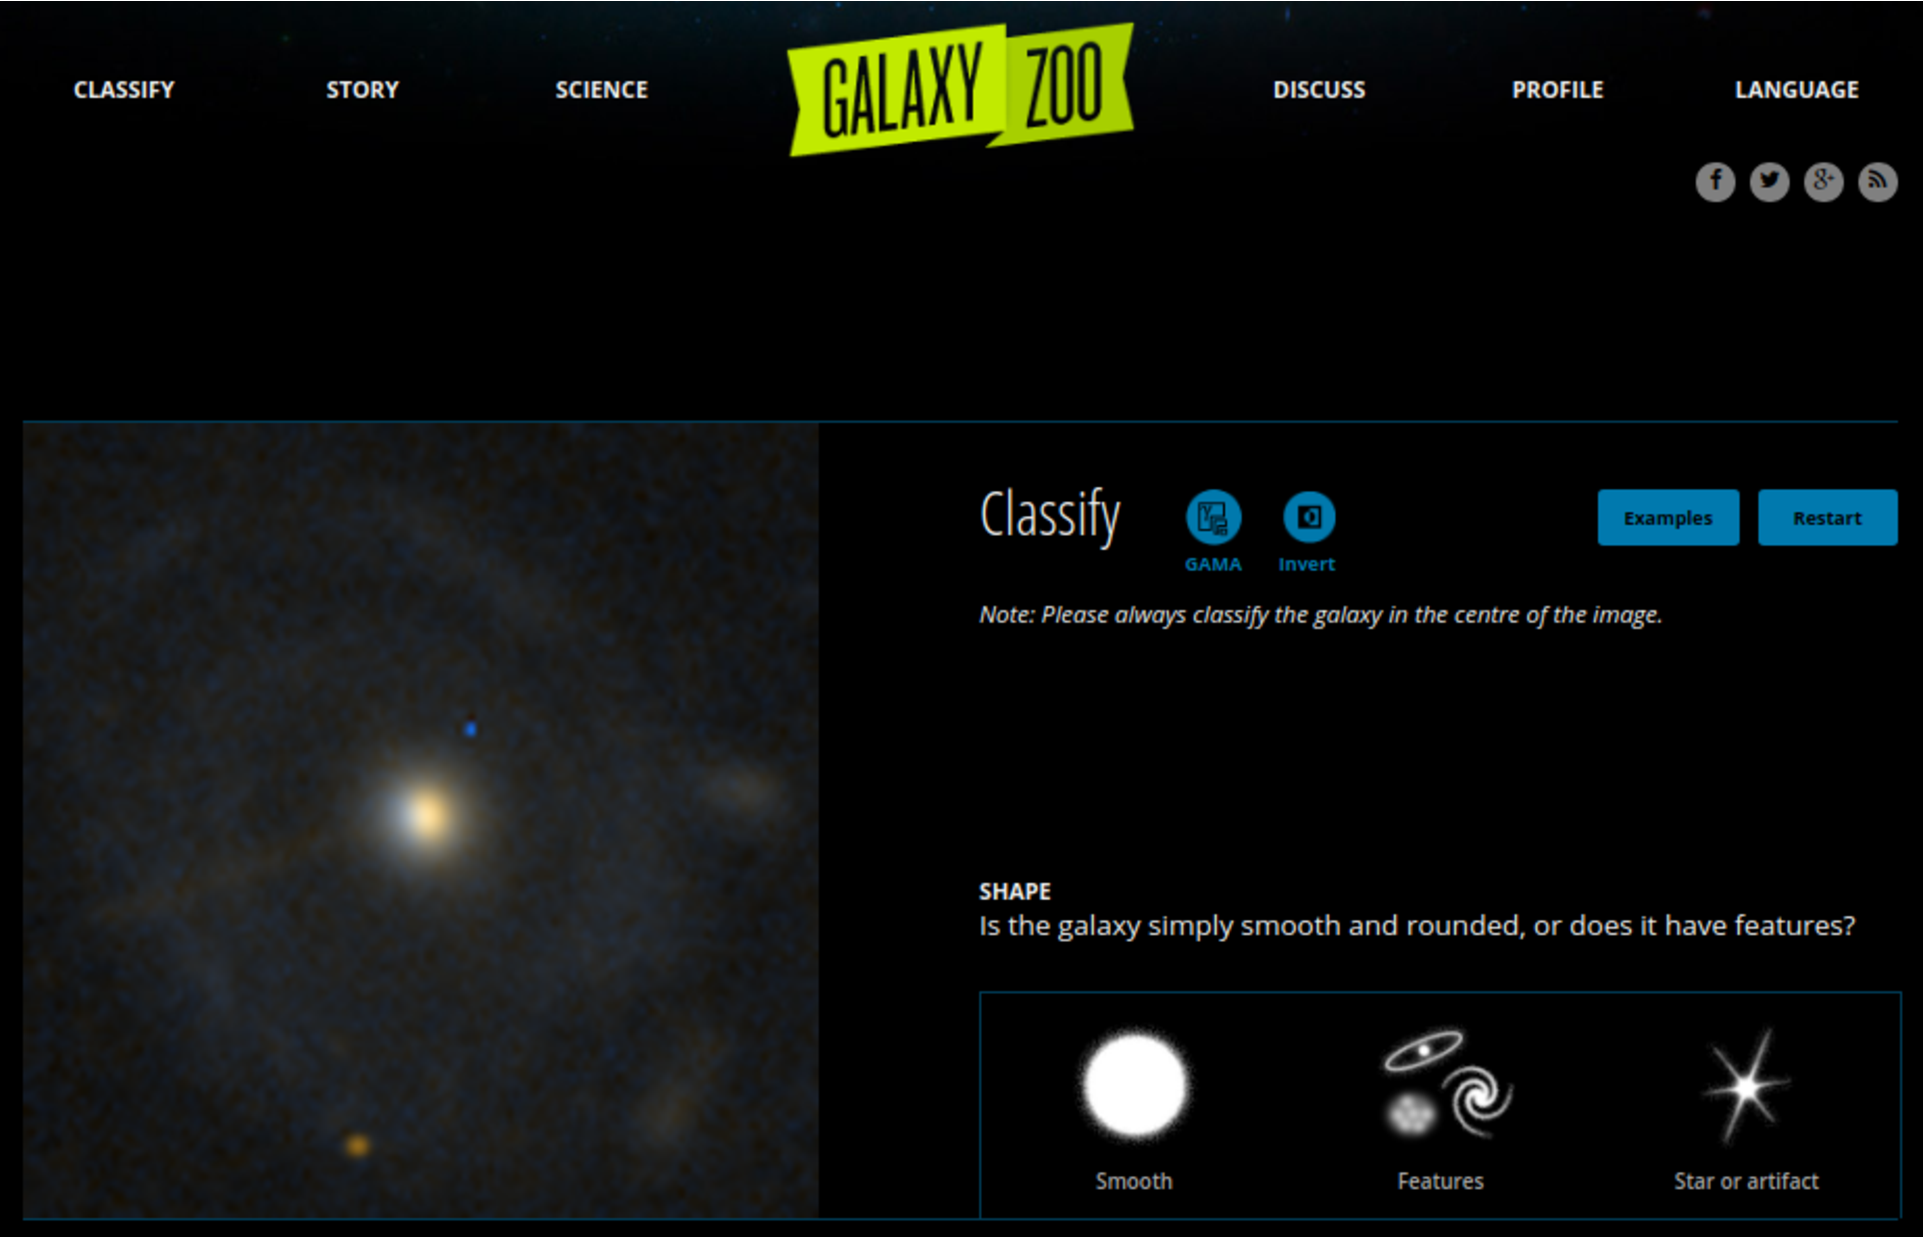
\includegraphics[width=\textwidth]{Figures/GZ2interface.pdf}
\caption{AHMAH MUTHAFUCKIN CAPTION BITCHES}
\label{fig: gz2 interface}
\end{figure}

%%%%%%%%%%%%%%%%%%%%%%%%%%%%%%%%%%%%%%%%%%%%%%%%%%%%%%%%%%%%%%%%%%%%%%%%%%
%%%		SUBSECTION: 	DATA REDUCTION
%%%%%%%%%%%%%%%%%%%%%%%%%%%%%%%%%%%%%%%%%%%%%%%%%%%%%%%%%%%%%%%%%%%%%%%%%%
\subsection{Data reduction}
The GZ2 catalog publishes several types of morphologies computed from volunteer classifications constisting of a vote fractrion for each response to every task, denoted $f_{\mathrm{response}}$. The most basic of these is computed simply as $f_r = n_r/n_t$, where $n_r$ is the number of votes of response $r$, and $n_t$ is the total number of votes for task $t$. In future chapters, this type of vote fraction is referred to as the \textit{raw} vote fraction as no post-processing has been performed. 

All GZ project perform a weighting scheme that evaulates the consistency of individual volunteers by assessing how their votes deviate from the majority for each task in the decision tree. This process effectively downweights volunteers whose responses are consistent with a random classifier. A volunteer's consistency, $\kappa$, for a given task is defined as 

\begin{equation}
\kappa = \frac{1}{N_r}\sum_{i=1}^{N_r}{\kappa_i}
\end{equation}
where $N_r$ is the total number of responses to a task, and $\kappa_i$ is $f_r$ if the volunteer's vote corresponds to response $i$, otherwise $\kappa=(1-f_r)$. Each volunteer is then assigned a mean consistency, $\bar\kappa$, which is the average consistency over all tasks. A weighting function is then applied according to  

\begin{equation}
w = \min({1.0, (\bar\kappa/0.6)^{8.5}}).
\end{equation}

All vote fractions are then recomputed using the volunteer weights and the process is repeated three times to assure convergence. The resulting vote fractions are dubbed \textit{weighted}. For GZ2, $w=1$ for $\sim$95\% of volunteers and thus the majority are treated equally. It's important to note that there is no up-weighting of exceptionally consistent volunteers.


Finally, when considering morphologies, be they visual or automatic, for a sample of galaxies in a small redshift range it is unlikely that galaxy evolution plays a major role in morphology variations. Thus, the presumed culprit is instead classification bias in that galaxies in the more distant universe tend to be, on average, smaller and dimmer. This obscures identification of features such as spiral arms, bars, and more. GZ2 corrects for this effect, briefly described below, producing \textit{debiased} vote fractions.

The general approach is such that, for a galaxy of a given size and brightness, a sample of other galaxies with similar characteristics will statistically share the same mix of morphologies. Thus the GZ2 main galaxy sample is binned by Petrosian absolute magnitude (M$_r$) and the Petrosian half-light radius, R$_{50}$,  as well as by redshift. A baseline morphology ratio is computed in the lowest redshift bin for those galaxies in the same with confirmed spectroscopic redshifts and with sufficient numbers of votes to yield statistically reliable classifications. This basiline is then used to correct more distant redshift bins. A more detailed account can be found in \cite{Willett2013}.

This thesis draws on the \textit{raw} vote fractions for reasons explained in Chapter \ref{chap:3}. Focus now turns to the methodology of measuring automatic morphological indictors which are used in Chapter \ref{chap:4} to train a machine classifier. 

%%%%%%%%%%%%%%%%%%%%%%%%%%%%%%%%%%%%%%%%%%%%%%%%%%%%%%%%%%%%%%%%%%%%%%%%%%
%%%		SECTION: 	AUTOMATIC MORPHOLOGY INDICATORS
%%%%%%%%%%%%%%%%%%%%%%%%%%%%%%%%%%%%%%%%%%%%%%%%%%%%%%%%%%%%%%%%%%%%%%%%%%
\section{Automatic morphology indicators}
Any machine classifier must have a set of features from which to learn to differentiate between classes. These features can be anything: pixel values, spectra, anything that can correlates well enough with the class boundary that the machine can learn that boundary. Choosing which features are most appropriate for each task is not necessarily straight-forward or easy. Too few features, and the machine will not be able to learn the things that define each class. Too many features and machine training time could increase substantially or, worse, training will be subjected to the Curse of Dimensionality: with increasing parameter space dimensionality, the number of samples required to learn that parameter space increases exponetially! 

In this work we draw on the Zurich Estimator of Structural Types (ZEST~\citep{Scarlata2007}). ZEST utilized five features measured from the light profile of galaxy imaging combined with a PCA analaysis to determine morphology for 120K COSMOS galaxies. These features are well known to correlate strongly with the distinction between early- and late-type galaxies. In this chapter we discuss how we measure these same features for the SDSS galaxy sample of GZ2. 

\subsection{Imaging data}
The Galaxy Zoo 2 galaxy sample was originally composed of 295305 subjects. However, the catalog paper published by \cite{Willett2013} provided classifications for only 285XXX. In a private conversation with the author, the remaining $\sim$10K galaxies in the GZ2 sample were unfit for classification for one reason or another and were thus excluded [is this because they were the galaxies with m$_r$ > 17.0??. However, as we explain in the next chapter, we use volunteer classifications from the original GZ2 database which includes classifications of these $\sim$10K galaxies. Because it is possible that these galaxies could have their morphology more accurately characterized by machine (as opposed to human classifications during the GZ2 project), thus obtaining SDSS imaging for the full GZ2 sample is attempted.  

$i$-band imaging (with central wavelength 7480\AA) from SDSS Data Release 12 is obtained for 290,059 galaxies in the GZ2 project. These are drawn from the meta data associated with each subject in the catalog of GZ2 galaxies which includes the RUN, CAMCOL, FIELD, etc, location indicators specificaly for SDSS imaging data. Because the original GZ2 project obtained imaging from DR7, it is surmised that the route to some galaxies in DR12 no longer exist thus explaining the loss of 5246 galaxy images. Because this represents such a small percentage [XXX] of the total population these galaxies were not tracked down at this time.

151,987 SDSS fields were successfully downloaded for the remaining galaxies in the sample. Because each SDSS field is $\sim$130 square arcminutes, most fields contain more than one galaxy in the GZ2 sample.  Postage stamps of each galaxy are cut from these fields where the dimensions of each cutout are 4$\times$Petrosian radius as measured by the SDSS pipeline. Galaxies located within 4 Petrosian radii of the edge of a field were excluded as image mosaicing was not performed. This removed 7962 galaxies from our sample resulting in a final sample of 282,350 GZ2 galaxy postage stamps. A random sample of these postage stamps is shown in Figure .  

\begin{figure}
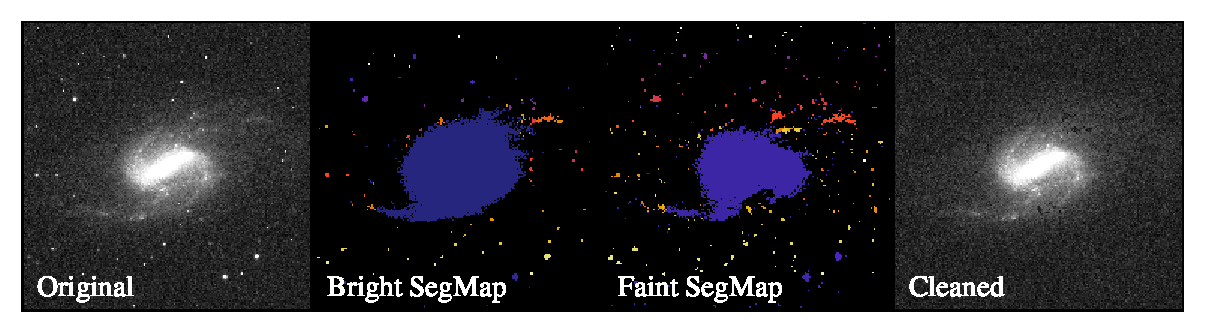
\includegraphics[width=\textwidth]{Figures/sextractor_example.pdf}
\caption{I'MMA FUCKING CAPTION BISH}
\label{fig: segmaps}
\end{figure}


\subsection{Image cleaning}
These postage stamps next undergo a cleaning process in order to remove the light from nearby sources so as not to contaminate the light profile of the galaxy of interest. Each stamp is processed through Source Extractor \citep[ver. 2.8.6;][]{sextractor}, a software that automatically detects sources in CCD imaging based on a set of input parameters that control its sensitivity. Two sets of parameters are used: the first is designed to identify bright sources while the second is better optimized to detect fainter objects. This software produces segmentation maps that identify the boundaries of each detected object in an image. By design, the galaxy of interest is located at the center of the cutout. Extraneous sources are then identifed from both the bright and faint segmentation maps and the pixels corresponding to these sources are replaced with a random value consistent with the background in that postage stamp.  An example of the segmentation maps created during this process is shown in Figure \ref{fig: segmaps}, while the first two columns in Figures XXX-XXX depict random samples of original and cleaned cutouts for a variety of ``difficulties''. To zeroth order, the difficulty of successfully cleaning an image of all stray light from other nearby sources is dependent upon how many other sources exist in the postage stamp and how close those sources are to the galaxy of interest. 


\begin{figure}
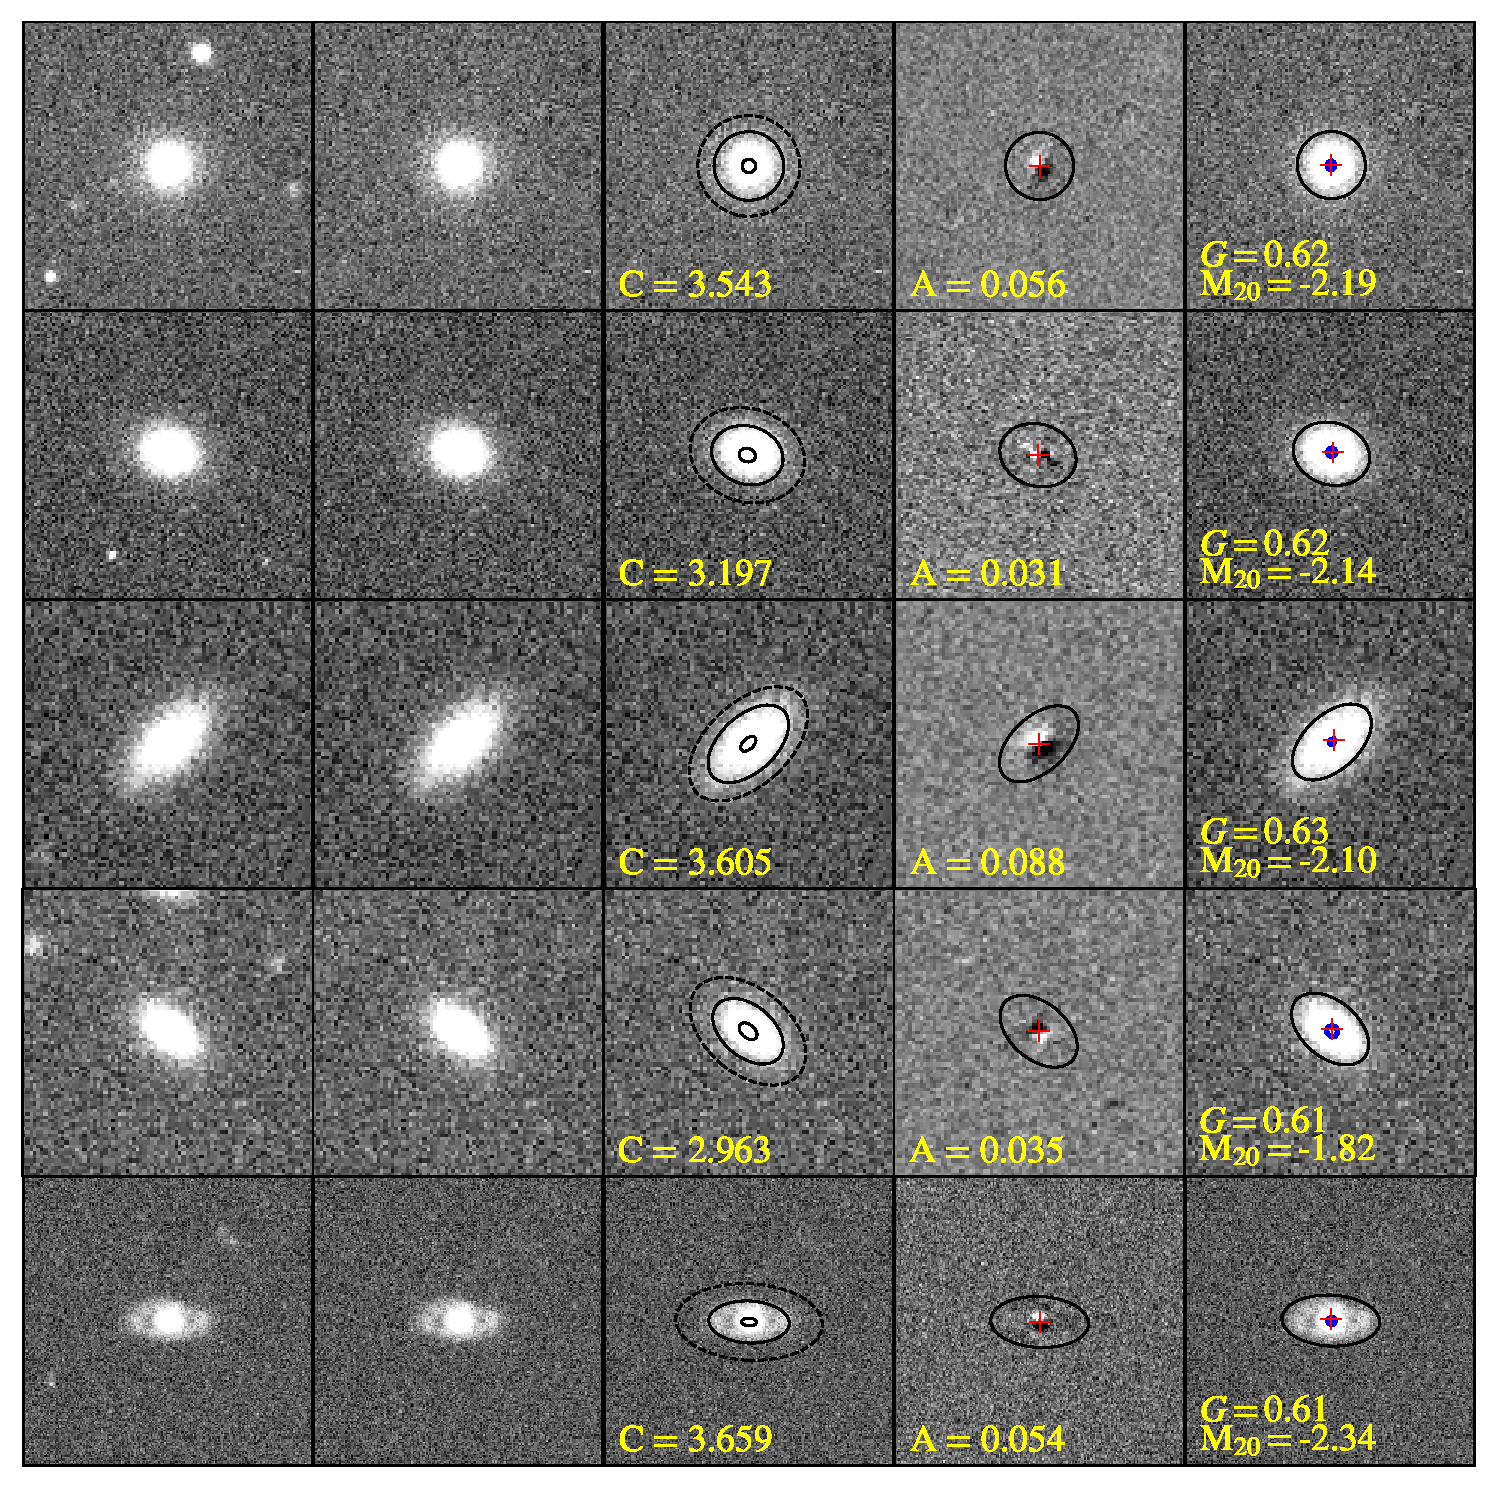
\includegraphics[width=\textwidth]{Figures/measure_morph_bin1.pdf}
\caption[Examples of image cleaning and morphology diagnostic measurements]{words words words I'm a fucking caption!}
\label{fig: clean examples}
\end{figure}

\begin{figure}
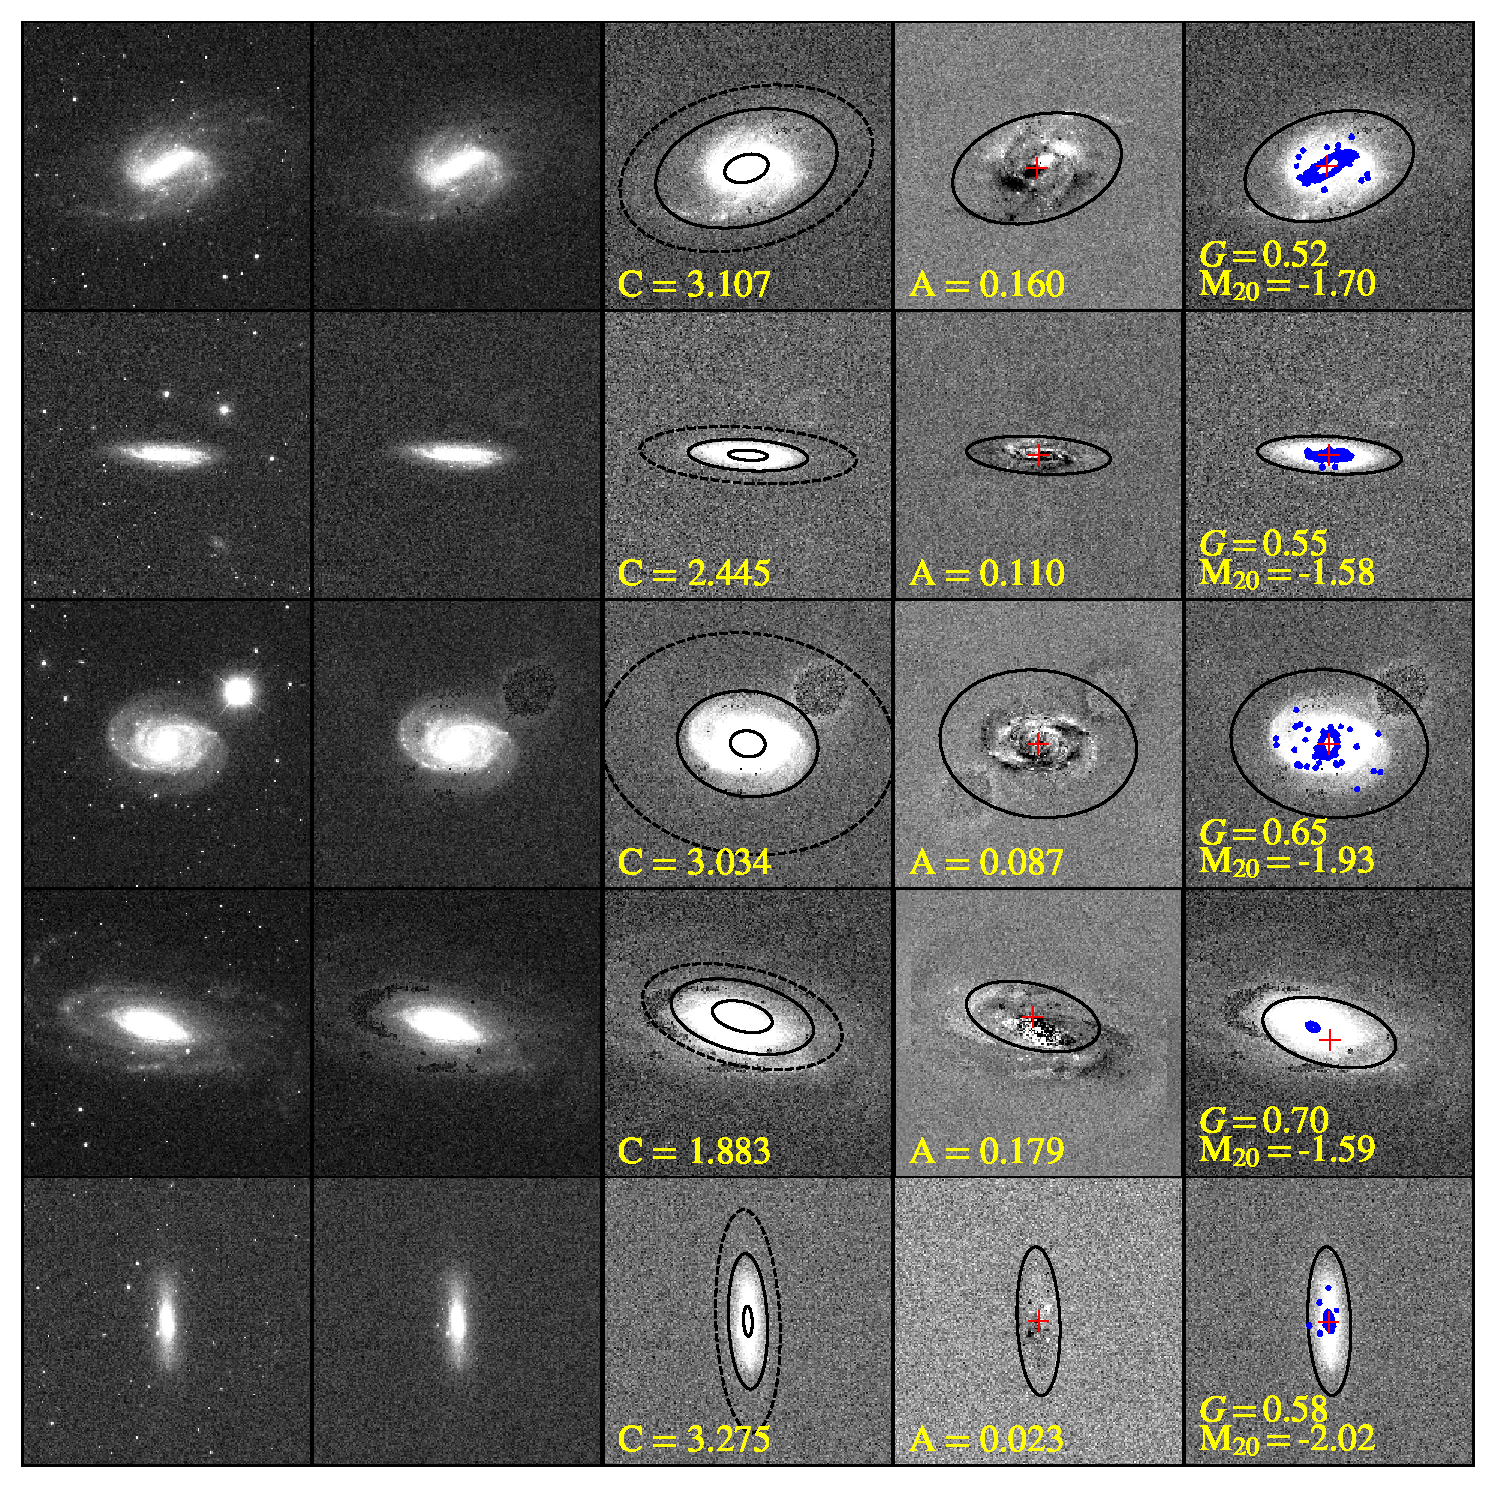
\includegraphics[width=\textwidth]{Figures/measure_morph_hardest.pdf}
\caption[Examples of image cleaning and morphology diagnostic measurements]{words words words I'm a fucking caption!}
\label{fig: clean examples}
\end{figure}


\subsection{Morphology indicators}
Defining the flux associated with a galaxy is a challenging task: galaxies do not have constant radial surface brightness, hard edges, or uniform shapes. Ideally, one would measure the total flux associated with a galaxy but this requires modelling of the light profile in addition to high signal-to-noise ratio in the outermost parts of the galaxy. Instead one could measure the flux within some isophote but unfortunately the fraction of light included within is dependent on the amplitude of the galaxy's surface brightness which diminishes due to cosmological redshift and Galactic extinction. To combat these issues, it is common practice to use the \cite{Petrosian1976} system  which is computes a radius defined by the empirical shape of the galaxy's light profile. Specifically, the Petrosian radius, $r_p$, is such that the ratio of the surface brightness at $r_p$ to the mean surface brightness within $r_p$ is equal to a fixed value $\eta$, i.e., 

\begin{equation}
\eta = \frac{\mu(r_p)}{\bar\mu(r<r_p)}
\end{equation}
where $\eta$ is traditionally set to 0.2. Because this is a ratio of surface brightnesses, cosmological factors affecting surface brightness no longer arise. 

In practice, $r_p$ is computed by first generating a set of elliptical annuli centered on the galaxy and equidistant in logspace. The number of annuli is determined by the size of the postage stamp. Elliptical apertures minimize the contribution from noisy background pixels. The position angle and galaxy center are taken from the SExtractor catalogs generated ealier. For each annulus, $\mu(r_i)$ is computed as the flux within the annulus divided by the annulus area, while $\mu(r<r_i)$ is computed as the total flux integrated to the center of that annulus divided by $\pi r_i^2$. This provides a crude estimate of $\eta$ which is then interpolated onto a finer set of radial values and $r_p$ is that radius for which the $eta$ intersects 0.2. Examples of surface brightness profilea are shown in Figure XXX. XX demonstrates a case in which the cleaning algorithm did not fully remove nearby contaminating light from other sources. This results in an $\eta$ that never crosses the 0.2 threshold. As a correction the excess light in the outer component is fit with a linear relation and a constant value subtracted from  the surface brightness profile. We next use these values of the Petrosian radius measured for X\% of our galaxies (\% catastrophic failures) to compute the following morphology diagnostics.

%We compute the following widely adopted nonparametric measurements of the galaxy light distribution on the cleaned postage stamps


%\subsubsection{Concentration}
Concentration is defined in several slightly different ways with the aim being to measure the ratio of the light within an inner aperture to that within an outer aperture. Small values of this ratio typically indicate disky galaxies, while larger values correlate with early-type ellipticals. We use the following definition \citep{Bershady2000}:

\begin{equation}{}
C = 5\log\Big(\frac{r_{80}}{r_{20}}\Big) 
\end{equation}
where \rr{80} and \rr{20} are the radii containing 80\% and 20\% of the total galaxy light respectively where we define the total flux as that within $r_p$ and the galaxy center is that determined by the asymmetry minimization \cite[described below,][]{Lotz2004}. A random sample of concentration measurements can be seen in the middle column of Figures XXX-XXX. 

The asymmetry parameter, $A$, quantifies the degree of rotational symmetry in the galaxy light distribution, not necessarily the physical shape of the galaxy as this is not highly sensitive to low surface brightness features. $A$ is measured by subtracting the galaxy image rotated by 180$^{\circ}$. A correction for background noise is applied (as in e.g.~\cite{Conselice2000, Lotz2004}), i.e., 
\begin{equation}
A = \frac{\sum_{x,y} |I(i,j) - I_{180}(i,j)|}{ 2\sum|I(i,j)|} - B_{180}
\end{equation}
where $I$ is the galaxy flux in each pixel $(x, y)$, $I_{180}$ is the image rotated by 180 degrees about the galaxy's central pixel, and $B_{180}$ is the average asymmetry of the background. $A$ is summed over all pixels within $r_p$ of the galaxy's center and then normalized by a corresponding measure in the original image. The center is determined by minimizing $A$ as described in \cite{Conselice2000}. Briefly, an initial central pixel is chosen and $A$ computed. Then asymmetry is calculated again in a $3\times3$ grid about that central pixel. If one of these produces a lower value of $A$, it becomes the new center and the process repeats until a minimum is found. This is a crucial step as \cite{Conselice2000} find that a small difference can change the asymmetry by up to 50\%. Additionally, the effects due to noise must also be corrected. This is accomplished by selecting a blank portion of the cutout with the same pixel area as defined for the $A$ measurement.  $A$ is computed as before, including the minimization, and this value then constitutes $B_{180}$. A random sample displaying the apertures and asymmetry centers are shown in the fourth columns of Figures XXX-XXX. 

The Gini coefficient, $G$, has long been used in econometrics as a measure of inequality by estimating the concentration of wealth in a nation's population. It is based on the Lorenz curve \citep{Lorenz1905} which is constructed by mapping the cumulative proportion of the population ranked by wealth onto the corresponding cumulative proportion of the size of their wealth. More formally, if $X$ is a positive random variable with cumulative distribution function $F(x)$ then the Lorenz curve goes as   
\begin{equation}
L(p) = \frac{1}{\bar X}\int^p_0 F^{-1}(u)~du,
\end{equation}
where $p$ is the percentile of the poorest denizens, and $\bar X$ is the mean over all values of $X_i$, a random deviate drawn from $X$. $G$ is then a summary statistic of this curve describing the mean of the absolute difference between all combinations of $X_i$:

\begin{equation}
G = \frac{1}{2\bar Xn(n-1)}\sum_{i=1}^n\sum_{j=1}^n\Big|X_i - X_j\Big|.
\end{equation}
This statistic was first applied to the distribution of a galaxy's light by \cite{Abraham2003} and further developed by \cite{Lotz2004}. In these terms, $G$ is 0 when the galaxy's flux is distributed homogeneously among all assigned pixels, and 1 if the light is concentrated within a single pixel. $G$ can be calculated more efficiently if the $X_i$ are first sorted into increasing order and then computing \citep{Glasser1962}
\begin{equation}
G = \frac{1}{|\bar X|n(n-1)}\sum_i^n(2i-n-1)|X_i|,
\end{equation}
where $n$ is the number of pixels assigned to the galaxy. Here we follow \cite{Lotz2004} by taking the absolute value of the flux, $X_i$, because in pixels with low signal-to-noise the flux is scattered to values below the mean sky level resulting in negative flux values for the faintest pixels. 

Assigning pixels to each galaxy must be given due consideration. As \cite{Lotz2004} point out, including too many sky pixels will systematically increase $G$, while exclusion of low surface brightness galaxy pixels will decrease $G$. \cite{Abraham2003} measure $G$ for pixels above a given surface brightness threshold but this will fall prey to cosmological effects. In this work, we compute $G$ from all pixels within $r_p$. This will exclude some low surface brightness features, especially for galaxies with faint, extended elements. However, this definition puts every galaxy on equal footing, and as explained in Chapter ???, any inherent systematics due to this choice will have little affect on the outcome of our machine learning algorithm. The last column in Figures XXX-XXX show examples of $G$.

%\subsubsection{M$_{20}$}
\M{20}~\citep{Lotz2004} is the second order moment of the brightest 20\% of the galaxy flux. It traces the spacial distribution of any bright galactic features such as nuclei, bars, spiral arms, or star-forming clusters. It is computed by first calculating the total moment as
\begin{equation}
 M_{\mathrm{tot}} = \sum_i^n M_i = \sum_i^nf_i[(x_i-x_c)^2 + (y_i-y_c)^2] 
\end{equation}
where $f_i$ is the flux in pixel $x_i$, $y_i$, and $x_c$, $y_c$ is the galaxy's center which is determined by minimizing $M_{tot}$ in a similar fashion as is done for the asymmetry. The galaxy pixels are then ranked by flux in descending order and $M_i$ is summed over the brightest pixels until that sum equals 20\% of the total galaxy flux, normalized by $M_{\mathrm{tot}}$:
\begin{equation}
 M_{20} = \log_{10} \Big( \frac{\sum_iM_i}{M_{\mathrm{tot}}} \Big), ~~\textrm{while} \sum_if_i < 0.2f_{\mathrm{tot}}
\end{equation}
where $f_{tot}$ is the total flux defined within $r_p$. For centrally concentrated objects, \M{20} correlates with $C$ but is also sensitive to bright off-centre knots of light. 

It's worth noting that both \M{20} and $G$ are correlated with $C$, but with key differences. Because $G$ is a measure of concentration it correlates strongly with $C$, especially for local galaxies \cite{Abraham2003}. However, $G$ is independent of spatial distribution: whereas $C$ measures the concentration in the central region of a galaxy, $G$ is sensitive to any concentration of light: centralized or not. M$_{20}$ takes this a step further with its key difference being a strong $r^2$ dependence. It is strongly weighted by the spatial distribution of bright regions but these need not be centralized either.  Indeed, when $G$ and \M{20} are taken together they are highly adept at identifying merging galaxies \citep{Lotz2004}.  


%\subsubsection{Ellipticity}
For our final morphology diagnostic, we use the ellipticity, $\epsilon = 1 - b/a$, of the light distribution as measured by SExtractor which computes the semi-major axis $a$ and semi-minor axis $b$ from the second-order moments of the galaxy light. The ellipticity of a galaxy correlates strongly with edge-on galaxies. 

In total, we measure morphological indicators for 282,350 SDSS galaxies. Some galaxies are lost at each stage of the measurement process due to various failures. For example, if the Petrosian radius is not well measured, no morphology diagnostics are computed for that galaxy. The number of galaxies measured for each of the morphology diagnostics is listed in Table \ref{tab:morph numbers}.  The relations between these diagnostics for the full sample is shown in Figure~\ref{fig: morph thresh}. The code developed to clean and compute these morphology indicators is open source and can be found at \url{https://github.com/melaniebeck/measure_morphology}.


% From the Selecting Random Subsamples for Thesis Chap3 (jupyter notebook)
\begin{table*}[]
	\centering
	\caption[Summary of morphology measurements]{}
	\label{tab:morph numbers}
	\let\mc\multicolumn
	\begin{tabular}{lcccc}
		\mc5c{ \textbf{Morphology measurement summary}} \\
		\hline \hline
		Full Galaxy Zoo 2 sample  & 	& 295305 &	 &   (\%) \\
		\hline
		Successful cutouts 		& 	& 282350 &	&	95.6 \\
		Petrosian radius		&	& 282334 &	&	95.6 \\
		Concentration			&	& 281957 &	&	95.5 \\
		M$_{20}$				&	& 282166 &	&	95.6 \\
		Asymmetry 				&	& 282269 &	&	95.3 \\
		Gini coefficient		&	& 282337 &	&	95.6 \\
		Ellipticity ($1 - b/a$)	&	& 282350 &	&	95.6 \\
		\hline
	\end{tabular}
\end{table*}

\subsection{Uncertainties and systematics}
Here goes all the stuff I've worked on this week. 

Gini coefficient sucks \citep{Lisker2008}.

\subsection{Comparison with other samples}
\begin{figure*}[t!]
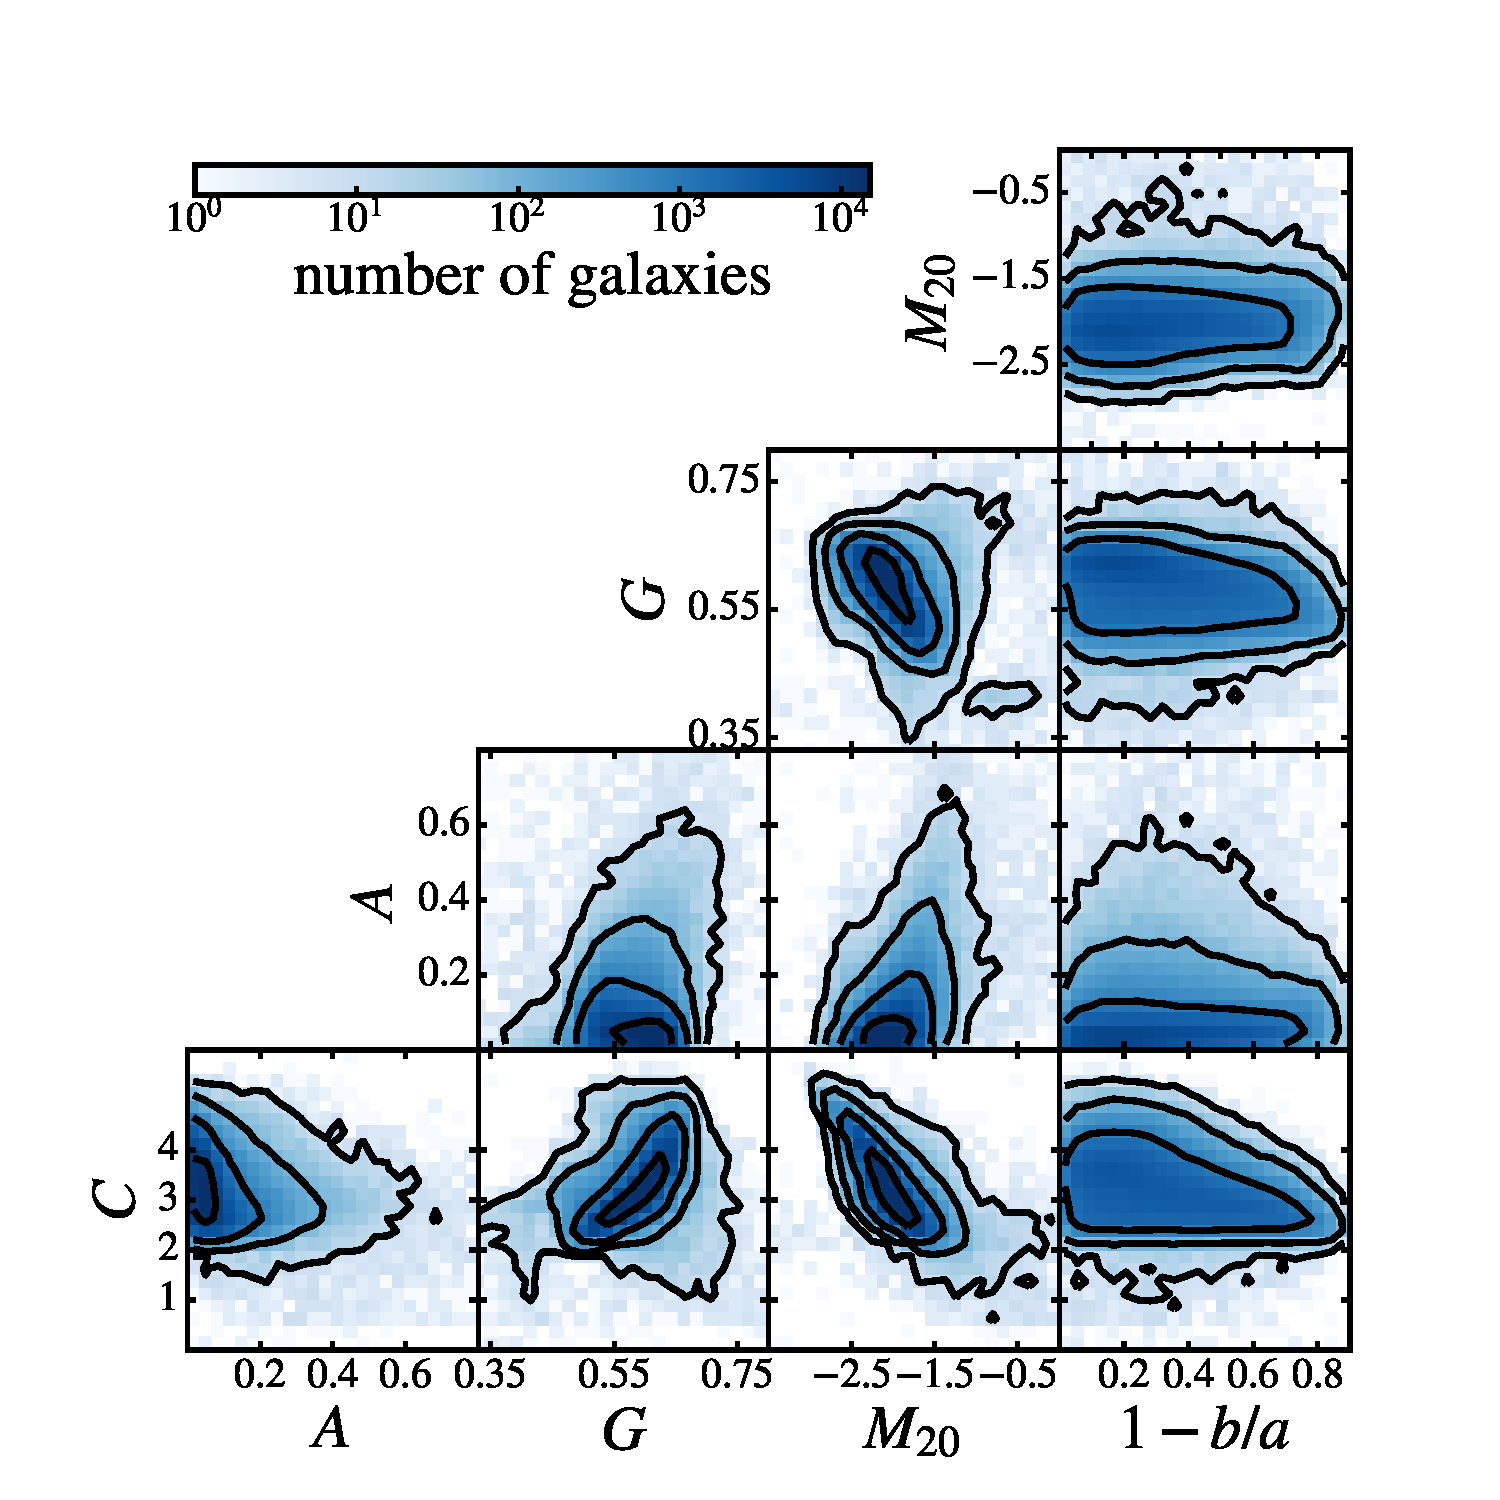
\includegraphics[width=3.7in]{Figures/human_machine/A2b.pdf}
\caption{\textit{Left.} Identifying~\feat~subjects is independent of identifying~\notfeat~subjects.  Both ROC curves use all subjects processed by SWAP where the score used to create the ROC curve is simply each subject's achieved posterior probability. The Featured curve demonstrates how well we identify~\feat~subjects with a threshold of 0.99, while the Not Featured curve demonstrates how well we identify~\notfeat~subjects with a threshold of 0.004. Typically, best performance is achieved by the score associated with the upper-left-most part of the curve. Our~\feat~threshold is nearly optimal, while our~\notfeat~threshold could be improved since the blue square is not as close to the upper left hand corner as other possible values of the subject posterior. \textit{Right.} Relation between measured morphology diagnostics for more than 280K SDSS galaxies. Most of these galaxies are processed through SWAP, receiving a posterior probability that estimates how likely each is to be~\feat~or~\notfeat.}
\label{fig: morph thresh}
\end{figure*}


Compare sample against sersic index, SDSS concentration, split by morphology, etc. 


\section{Catalog of morphological indicators for 282350 SDSS galaxies}
Put in a big table here with a subsample of the catalog? Link to somewhere online where the rest of the catalog can be found? 


\begin{deluxetable}{lccccccccc}
\rotate
\tablecolumns{10}
\tablewidth{0pt}
\tablecaption{Morphology Diagnostics for $\sim$283K SDSS Galaxies in the GZ2 Sample}
\tablehead{
	\colhead{DR7 objID} &
	\colhead{RA}		&
	\colhead{DEC}		&
	\colhead{R$_p$}		&
	\colhead{$C$}		&
	\colhead{$A$}		&
	\colhead{\M{20}}	&
	\colhead{$G$}		&
	\colhead{e}			&
	\colhead{flags}		
}
\startdata
587722981736054938 & 170.749 &	-1.25746 &	44.09 & 2.556 & 0.0243 & -1.888 & 0.539 & 4.289 &	\\
\enddata
\end{deluxetable}